\section{Results}\label{sec:results}

\textbf{[DISCUTIR E ESCREVER: cada tabela com uma infer\^encia; tirar do texto os n\'umeros que j\'a est\~ao nas tabelas.]}

\subsection{Size, payment and recovery}\label{sec:size}

Assessed debt is the value. Declared debt is the count.
Table~\ref{tab:profile} puts the two segments on the same December 2025 definitions.
Assessed certificates are few and large.
Declared certificates are many and small.
The median assessed certificate is \brl{}578,084 and the median declared certificate is \brl{}7,334.
At the firm, the medians are \brl{}770,756 and \brl{}7,916.
The rank-biserial correlation is 0.89 at the certificate and 0.74 at the firm (Table~\ref{tab:mw}).
Both are large.
The first expectation, that assessments would pick out larger balances, is met in the cross-section.
The second is met as well.
Declared debt is 97.4~percent of the two-segment certificates and 27.2~percent of the two-segment stock.

Payment and recovery do not agree.
A payment occurs on 17.4~percent of assessed certificates and on 9.1~percent of declared certificates.
Recovery, payments divided by the December stock, is 0.48~percent for assessed debt and 4.73~percent for declared debt.
In reais, payments before 2026 are \brl{}5.50 billion on declared debt and \brl{}1.49 billion on assessed debt.
Declared debt is 27.2~percent of the two-segment stock and 78.7~percent of the two-segment payments.
The third expectation was that these two rates need not rank the segments together.
They do not.
Some payment is more common on the assessed side.
Reais collected per real of stock are higher on the declared side, where the balances are smaller.

\begin{table}[t]
\centering
\caption{Declared and assessed \vat{} debt in December 2025.}\label{tab:profile}
\begin{tabular}{lrr}
\toprule
& Declared & Assessed \\
\midrule
Certificates & 2,257,189 & 59,542 \\
Firms (CNPJ root) & 177,682 & 30,005 \\
Stock (\brl{} billion) & 116.42 & 311.40 \\
Median certificate (\brl{}) & 7,334 & 578,084 \\
Median firm stock (\brl{}) & 7,916 & 770,756 \\
Certificates with any payment (\%) & 9.1 & 17.4 \\
Recovery, payments / stock (\%) & 4.73 & 0.48 \\
Payments before 2026 (\brl{} billion) & 5.50 & 1.49 \\
Share of two-segment stock (\%) & 27.2 & 72.8 \\
Share of two-segment payments (\%) & 78.7 & 21.3 \\
Median debt age, certificate (years) & 4.7 & 9.3 \\
Median debt age, firm (years) & 2.1 & 8.9 \\
Stock enrolled more than 10 years (\%) & 39.5 & 43.7 \\
\bottomrule
\end{tabular}

\vspace{0.4em}
\begin{minipage}{0.95\textwidth}
\footnotesize
Notes: Legal entities. Stock is the December 2025 value net of legal fees.
Payments are GARE amounts dated before 1~January 2026.
Firm debt age is the stock-weighted mean age of the firm's certificates in the segment.
The share older than 10 years uses certificate stock with a usable enrolment date.
\end{minipage}
\end{table}

\begin{table}[t]
\centering
\caption{Mann--Whitney comparisons of assessed and declared debt.}\label{tab:mw}
\begin{tabular}{llrrr}
\toprule
Outcome & Unit & Median assessed & Median declared & Rank-biserial \\
\midrule
Stock & Certificate & \brl{}578,084 & \brl{}7,334 & 0.89 \\
Stock & Firm & \brl{}770,756 & \brl{}7,916 & 0.74 \\
Debt age (years) & Certificate & 9.3 & 4.7 & 0.39 \\
Debt age (years) & Firm & 8.9 & 2.1 & 0.55 \\
Firm age (years) & Certificate & 25.3 & 18.3 & 0.30 \\
Firm age (years) & Firm & 24.1 & 13.4 & 0.45 \\
\bottomrule
\end{tabular}

\vspace{0.4em}
\begin{minipage}{0.95\textwidth}
\footnotesize
Notes: A positive rank-biserial correlation means a random assessed unit tends to exceed a random declared unit.
Stock comparisons use positive values (59,294 assessed certificates and 2,254,387 declared certificates).
Firm age is defined on establishment matches.
Every $p$-value is zero at floating-point precision and is omitted.
\end{minipage}
\end{table}

\subsection{Concentration and the 1~percent cut}\label{sec:conc}

The pooled book is highly concentrated, and the concentration is an assessed tail.
Figure~\ref{fig:lorenz} plots the Lorenz curves.
Table~\ref{tab:top1} reports the upper tail at several cuts.
On positive values, the pooled Gini coefficient is 0.946.
The largest 10~percent of certificates hold 91.9~percent of the stock, the largest 5~percent hold 87.5~percent, the largest 1~percent hold 75.8~percent, and the largest 0.1~percent hold 48.5~percent.
The largest half of certificates hold 99.4~percent.
The curve therefore stays near zero and then rises at the right edge.

The largest 1~percent of certificates is a natural cut in this portfolio for two reasons that point the same way, and for a third fact that limits what the cut means.
First, on the pooled book the Lorenz curve stays close to zero over most of the distribution and rises sharply only in the extreme tail, so the largest 1~percent (23,137 certificates) already hold three quarters of the stock.
Second, a review list of that order of magnitude is an administrative object.
The attorney office can assign specialised collection to a set of about 23,000 certificates, and that set contains three quarters of the stock.
Third, the same cut does not mean that each segment is equally concentrated.
Inside declared debt the largest 1~percent hold 39.5~percent of declared stock, and inside assessed debt they hold 39.9~percent.
The pooled 75.8~percent appears because assessed debt is 72.8~percent of the two-segment stock and only 2.6~percent of the certificates.
Of the 23,137 certificates in the pooled top 1~percent, 18,230 are assessed and account for 68.8~percent of the pooled stock.
The other 4,907 are declared and account for 7.1~percent.
The cut is therefore a description of where the money sits.
It is not evidence that collecting those certificates would recover the stock, and it is not a within-segment law.

Inside trade and inside manufacturing, the largest 1~percent of certificates still hold between 35 and 42~percent of that section's own stock.
The within-section Gini coefficients are about 0.82 to 0.87.
Moving down the activity classification does not reproduce the pooled 75.8~percent.
That figure is the mixture of the two segments.

\begin{figure}[t]
\centering
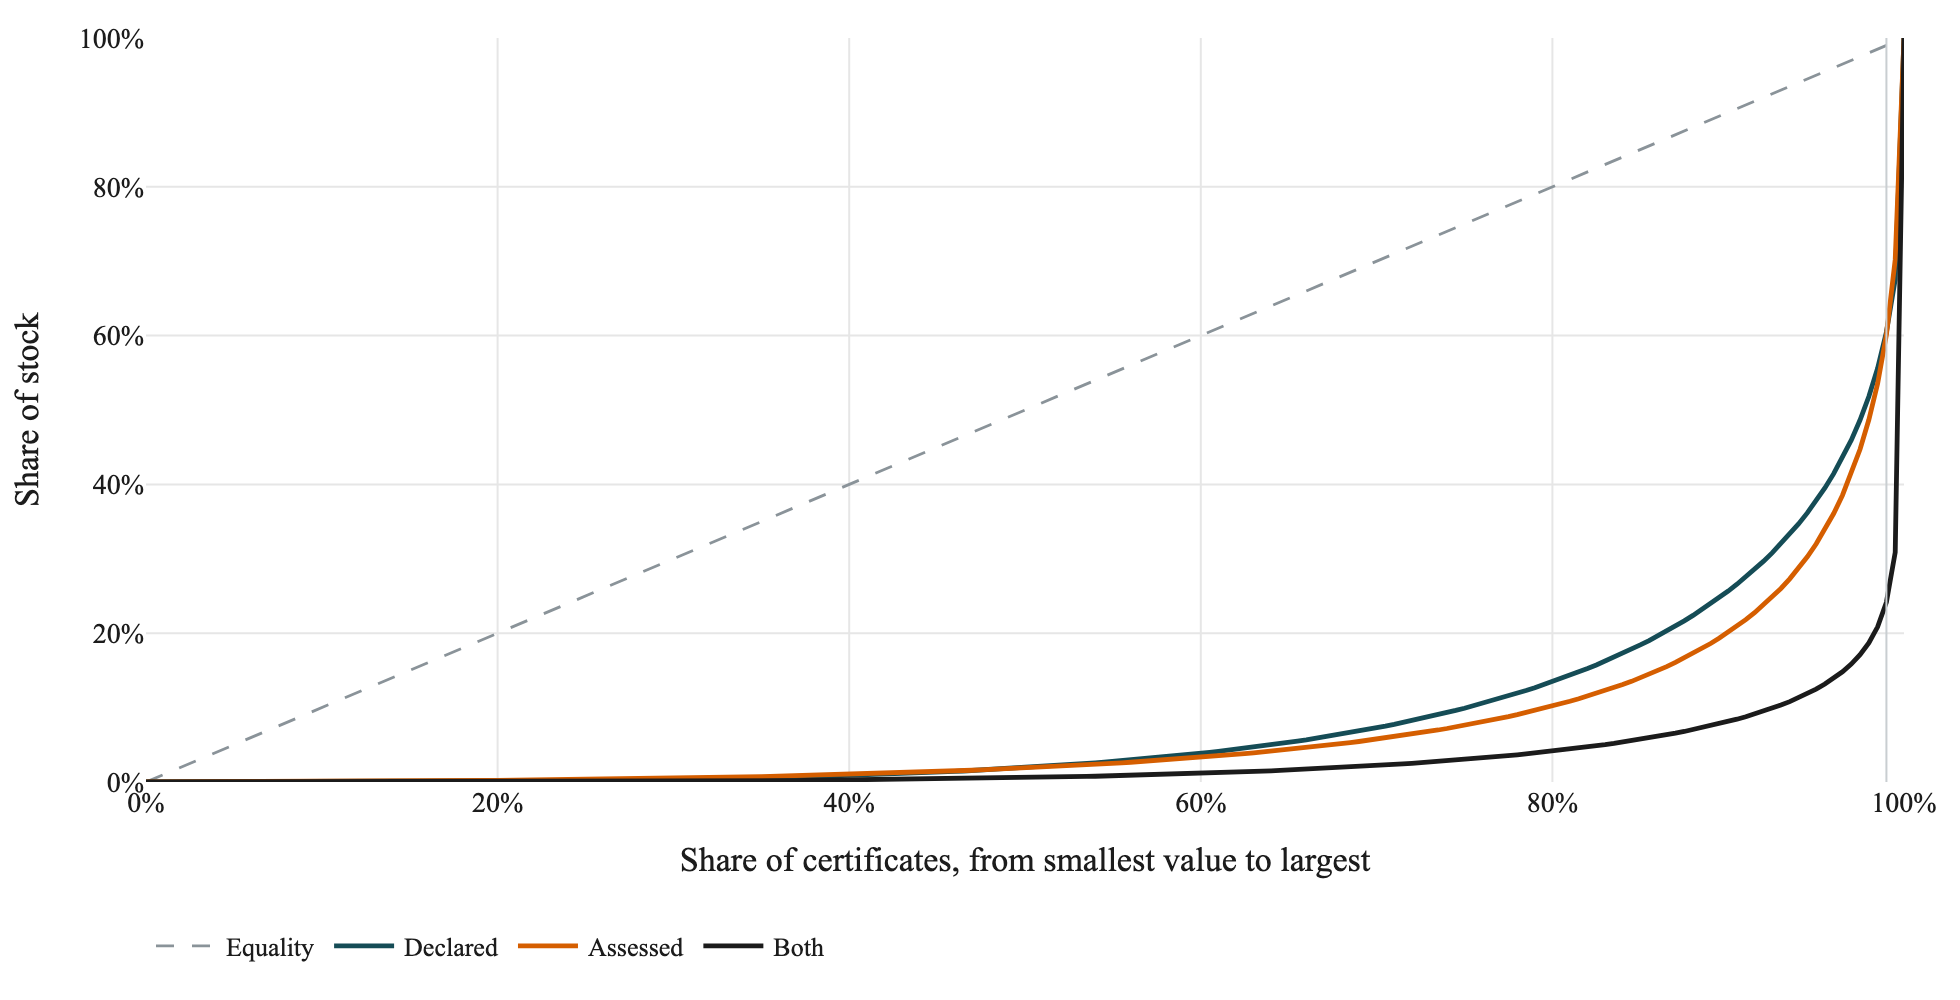
\includegraphics[width=\textwidth]{figures/fig_lorenz_segment.png}
\caption{Lorenz curves of December 2025 stock, positive certificate values.}\label{fig:lorenz}
\end{figure}

\begin{table}[t]
\centering
\caption{Upper tail of the pooled stock, and the same 1~percent cut inside each segment.}\label{tab:top1}
\begin{tabular}{lrrr}
\toprule
Cut, from the largest certificates & Certificates & Share of certificates (\%) & Share of stock (\%) \\
\midrule
\multicolumn{4}{l}{\textit{Pooled book}} \\
Largest 10 percent & 231,369 & 10 & 91.9 \\
Largest 5 percent & 115,685 & 5 & 87.5 \\
Largest 1 percent & 23,137 & 1.00 & 75.8 \\
Largest 0.5 percent & 11,569 & 0.5 & 69.1 \\
Largest 0.1 percent & 2,314 & 0.1 & 48.5 \\
\addlinespace
\multicolumn{4}{l}{\textit{Inside each segment, largest 1 percent}} \\
Declared & 22,544 & 1.00 & 39.5 \\
Assessed & 593 & 1.00 & 39.9 \\
\bottomrule
\end{tabular}

\vspace{0.4em}
\begin{minipage}{0.95\textwidth}
\footnotesize
Notes: Positive values only.
The pooled Gini coefficient is 0.946.
Inside the segments it is 0.839 (declared) and 0.863 (assessed).
Of the 23,137 pooled top-1~percent certificates, 18,230 are assessed and hold 68.8~percent of the pooled stock.
\end{minipage}
\end{table}

\subsection{Age of the debt and age of the firm}\label{sec:age}

Assessed debt is older, and the firms that hold it are older.
The median declared certificate is 4.7 years from enrolment.
The median assessed certificate is 9.3 years.
The rank-biserial correlation is 0.39.
At the firm, using the stock-weighted age, the medians are 2.1 and 8.9 years and the correlation is 0.55.
The share of stock older than 10 years is closer: 39.5~percent declared and 43.7~percent assessed.
The age gap is in the centre of the distribution more than in the extreme tail.
Figure~\ref{fig:age} shows the stock shares by band.

Firm age lines up in the same direction.
The median firm is 13.4 years old on the declared side and 24.1 years old on the assessed side (rank-biserial correlation 0.45).
Firms aged 20 years or more hold 66.3~percent of declared stock and 76.0~percent of assessed stock.
Young firms hold little of either stock.
This is consistent with assessment falling on established operations, and with declared debt tracking a wider filing population.
It is not a finding about survival, because we see the register once.

\begin{figure}[t]
\centering
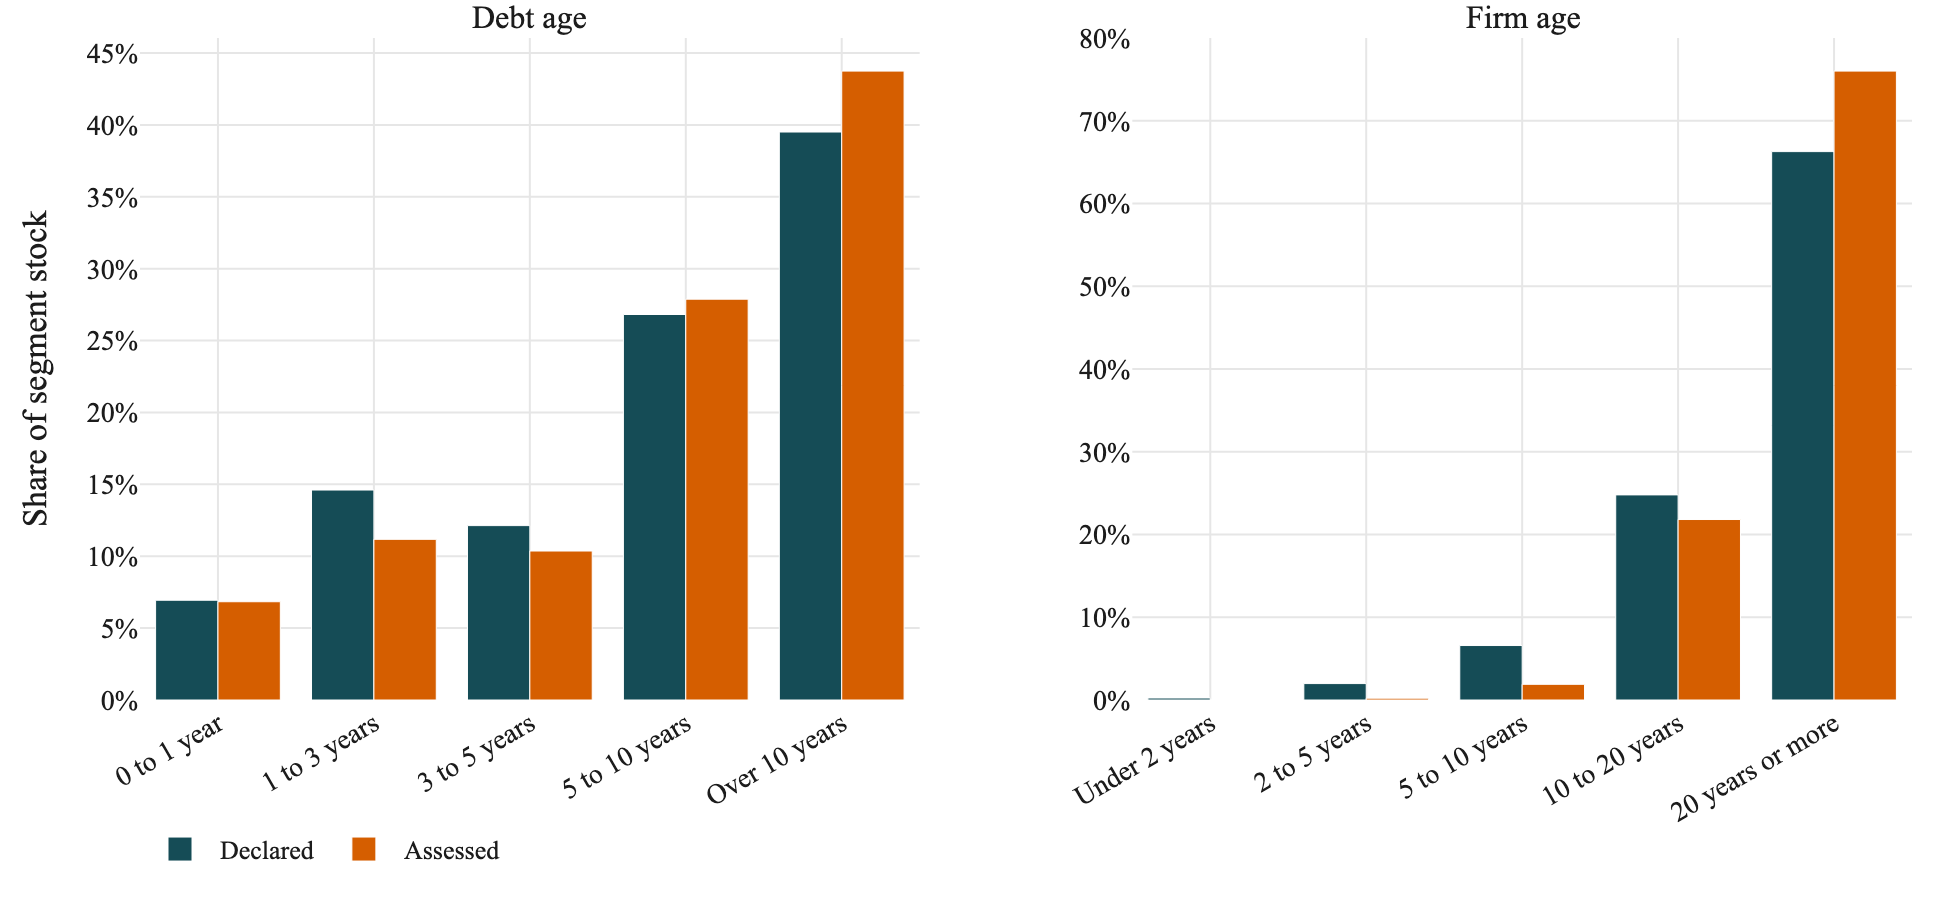
\includegraphics[width=\textwidth]{figures/fig_age_bands.png}
\caption{Share of segment stock by debt age and by firm age, 31~December 2025.}\label{fig:age}
\end{figure}

\subsection{Activity, status, size, place and repeated certificates}\label{sec:firms}

The activity mix differs in the stock even though the association across firms is small.
Cram\'er's $V$ for CNAE section, on one row per firm, is 0.10 (Table~\ref{tab:attr}).
Figure~\ref{fig:section} shows why the stock can still look different.
Trade is 45.4~percent of assessed stock and 27.6~percent of declared stock.
Manufacturing is 34.5~percent and 50.8~percent.
Transport is 4.6~percent and 12.5~percent.
Information is 6.0~percent and 0.8~percent.
Table~\ref{tab:section} reports payment and recovery for these sections.
In each of them, the payment rate is higher for assessed certificates and the recovery rate is higher for declared certificates.
The ranking in Section~\ref{sec:size} is not an artefact of one sector.

Divisions make the same contrast more specific (Table~\ref{tab:division}).
Wholesale trade, except motor vehicles, is 32.0~percent of assessed stock and 14.4~percent of declared stock.
Telecommunications is 5.5~percent and 0.5~percent.
Coke and petroleum products are 9.8~percent of declared stock and 1.4~percent of assessed stock.
Land transport is 11.7~percent and 3.3~percent.
Retail is large on both sides, at about 12~percent of each stock, with the same payment-versus-recovery pattern.

Registry status is the stronger categorical difference.
$V$ is 0.25.
Active firms hold 74.4~percent of declared stock and 52.9~percent of assessed stock.
Closed firms hold 9.7~percent and 24.1~percent.
Unfit firms hold 15.2~percent and 21.7~percent (Figure~\ref{fig:status}).
Size is milder ($V = 0.18$).
Firms outside the micro and small categories hold 74.1~percent of declared stock and 81.6~percent of assessed stock.
Small firms hold 15.3~percent and 7.6~percent.
Legal form is similar in the stock.
A limited company holds 77.8~percent of declared stock and 77.0~percent of assessed stock, and $V$ for legal nature is 0.12.

Geography is dominated by S\~ao Paulo, with a larger out-of-state share on the declared side ($V = 0.15$).
S\~ao Paulo state is 95.7~percent of assessed stock and 88.0~percent of declared stock.
Rio de Janeiro state is 1.5~percent and 8.2~percent.
The city of S\~ao Paulo holds 27.2~percent of assessed stock and 22.5~percent of declared stock.
The city of Rio de Janeiro holds 7.8~percent of declared stock.
Paul\'inia, with 215 firms, holds 4.9~percent of assessed stock.

Repeated enrolment is common, and it is not the same fact in the two segments ($V = 0.26$ on the firm-by-segment table).
On the declared side, 119,833 firms have two or more certificates.
They are 67.4~percent of declared firms and hold 99.2~percent of declared stock.
On the assessed side, 9,565 firms have two or more certificates.
They are 31.9~percent of assessed firms and hold 82.3~percent of assessed stock (Figure~\ref{fig:repeated}).
A single assessed certificate is therefore a larger part of the assessed firm count than a single declared certificate is of the declared firm count.
The declared stock barely exists outside multi-certificate firms.
Separately, 11,928 firms hold at least one certificate in each segment.
The attribute tests assign each of those firms to the segment with the larger stock.
The repeated-enrolment counts do not.
They describe each book on its own.

\begin{table}[t]
\centering
\caption{Firm-level associations between segment and debtor attributes.}\label{tab:attr}
\begin{tabular}{lrr}
\toprule
Attribute & Firms in the test & Cram\'er's $V$ \\
\midrule
CNAE section & 195,759 & 0.10 \\
Legal nature & 195,759 & 0.12 \\
State (UF) & 195,759 & 0.15 \\
Firm size & 195,759 & 0.18 \\
Registry status & 195,759 & 0.25 \\
Repeated enrolment & 207,687 & 0.26 \\
\bottomrule
\end{tabular}

\vspace{0.4em}
\begin{minipage}{0.95\textwidth}
\footnotesize
Notes: Chi-square tests on firm counts.
Except for repeated enrolment, each CNPJ root is placed in the segment that holds more of its stock.
The repeated-enrolment row counts a firm once in each segment in which it has a certificate.
Every $p$-value is zero at floating-point precision.
\end{minipage}
\end{table}

\begin{figure}[t]
\centering
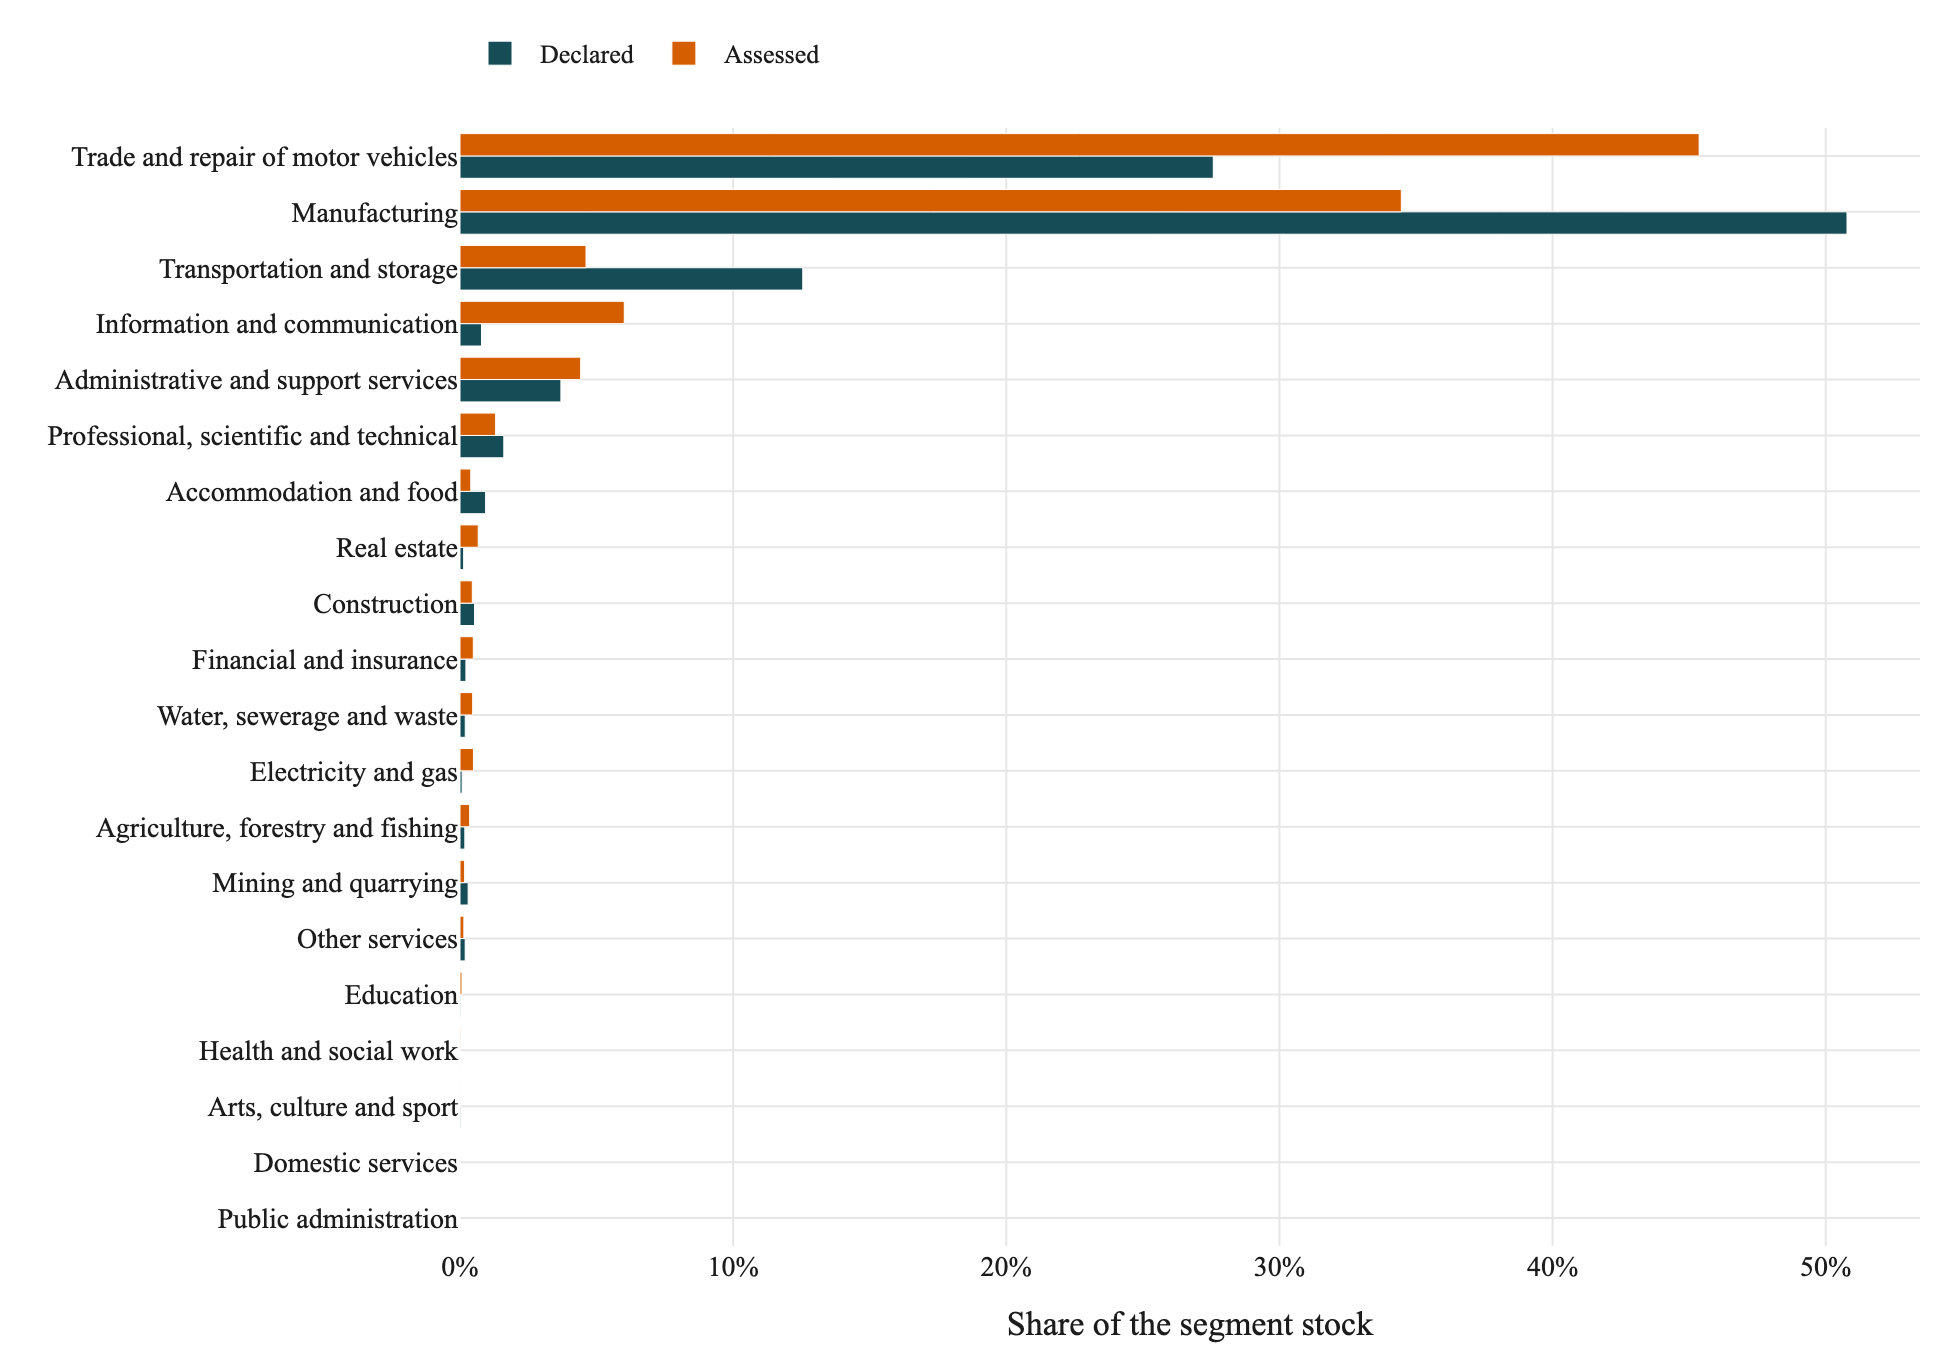
\includegraphics[width=\textwidth]{figures/fig_cnae_section.png}
\caption{Share of segment stock by CNAE section.}\label{fig:section}
\end{figure}

\begin{table}[t]
\centering
\small
\caption{Main CNAE sections: stock, payment and recovery by segment.}\label{tab:section}
\begin{tabular}{lrrrrrr}
\toprule
& \multicolumn{2}{c}{Share of segment stock (\%)} & \multicolumn{2}{c}{Any payment (\%)} & \multicolumn{2}{c}{Recovery (\%)} \\
\cmidrule(lr){2-3}\cmidrule(lr){4-5}\cmidrule(lr){6-7}
Section & Declared & Assessed & Declared & Assessed & Declared & Assessed \\
\midrule
Manufacturing & 50.8 & 34.5 & 9.6 & 16.6 & 4.81 & 0.51 \\
Trade and repair of vehicles & 27.6 & 45.4 & 7.8 & 17.4 & 4.46 & 0.39 \\
Transportation and storage & 12.5 & 4.6 & 12.3 & 21.5 & 4.69 & 0.90 \\
Information and communication & 0.8 & 6.0 & 11.3 & 16.9 & 5.88 & 0.84 \\
Administrative and support & 3.7 & 4.4 & 10.3 & 18.5 & 5.59 & 0.33 \\
Professional services & 1.6 & 1.3 & 10.1 & 19.0 & 1.70 & 0.16 \\
All other sections & 3.0 & 3.8 &  &  &  &  \\
\bottomrule
\end{tabular}

\vspace{0.4em}
\begin{minipage}{0.95\textwidth}
\footnotesize
Notes: Sections shown are those with at least 1~percent of either segment's stock.
Payment and recovery for the residual row are omitted because the row mixes unlike activities.
Short English names render the official Portuguese section titles.
\end{minipage}
\end{table}

\begin{figure}[t]
\centering
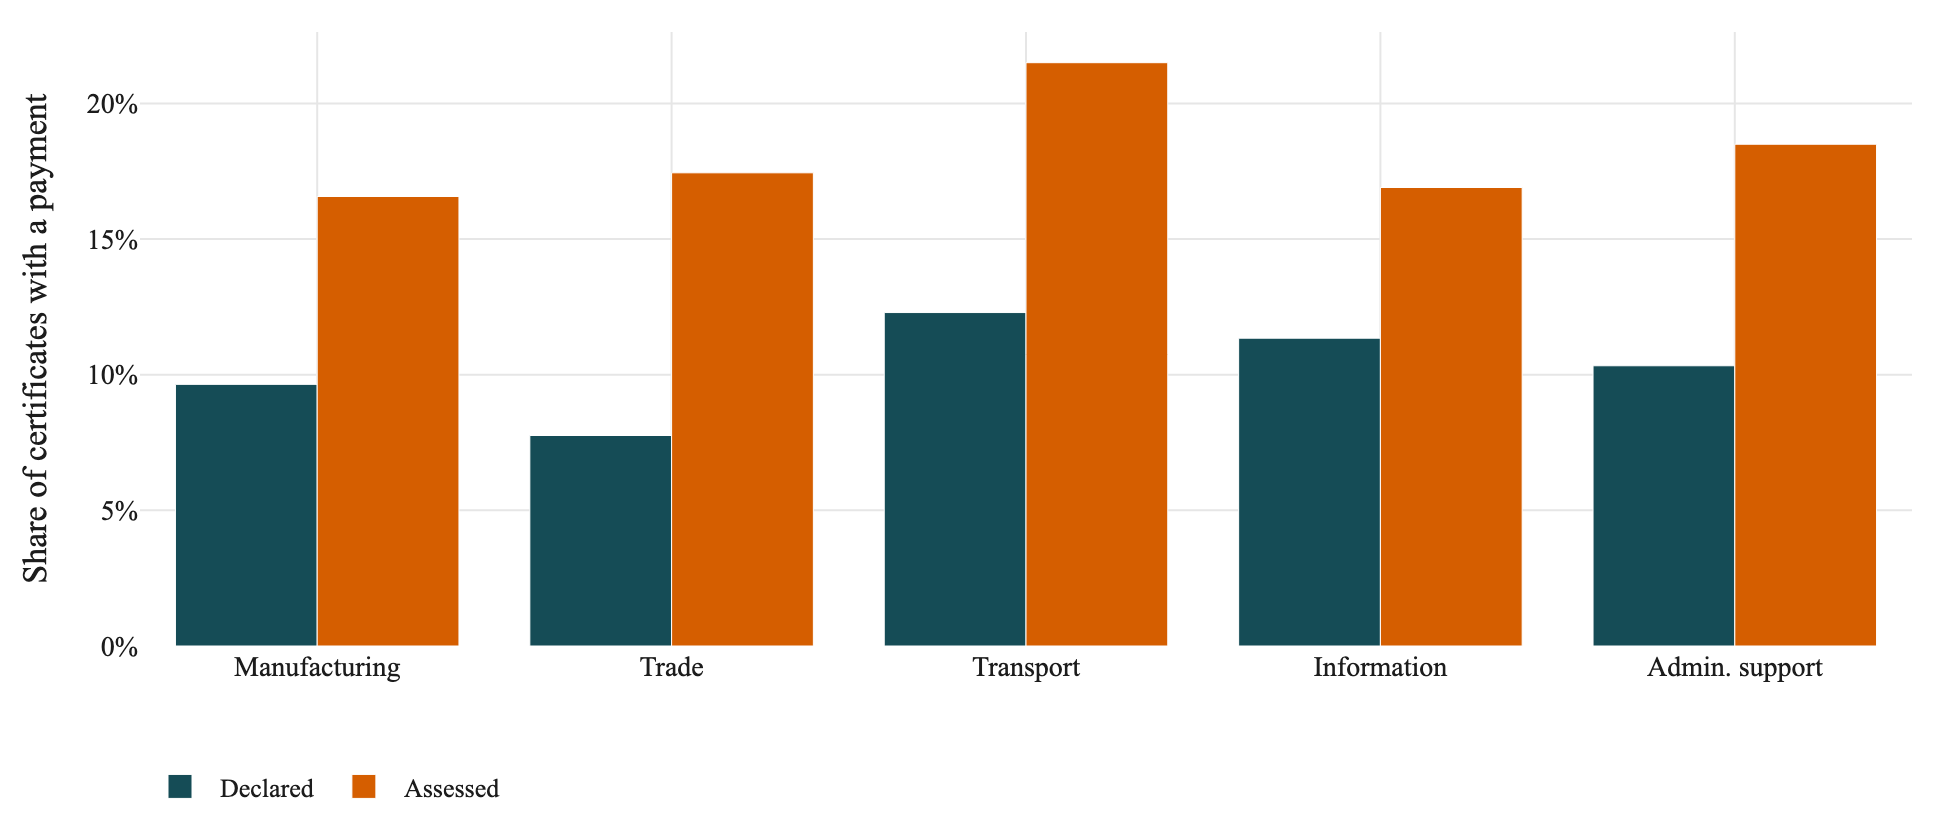
\includegraphics[width=\textwidth]{figures/fig_payment_section.png}
\caption{Share of certificates with any payment, sections with at least 2~percent of a segment's stock.}\label{fig:payment}
\end{figure}

\begin{table}[t]
\centering
\small
\caption{Selected CNAE divisions by share of segment stock.}\label{tab:division}
\begin{tabular}{llrrrr}
\toprule
Code & Division & \multicolumn{2}{c}{Share of stock (\%)} & \multicolumn{2}{c}{Recovery (\%)} \\
\cmidrule(lr){3-4}\cmidrule(lr){5-6}
& & Declared & Assessed & Declared & Assessed \\
\midrule
46 & Wholesale, except vehicles & 14.4 & 32.0 & 4.21 & 0.30 \\
47 & Retail trade & 12.0 & 11.8 & 4.85 & 0.60 \\
49 & Land transport & 11.7 & 3.3 & 4.53 & 1.18 \\
19 & Coke and petroleum products & 9.8 & 1.4 & 1.37 & 0.41 \\
10 & Food products & 4.3 & 7.4 & 7.02 & 0.45 \\
61 & Telecommunications & 0.5 & 5.5 & 6.73 & 0.88 \\
24 & Basic metals & 2.0 & 4.7 & 5.22 & 0.35 \\
\bottomrule
\end{tabular}

\vspace{0.4em}
\begin{minipage}{0.95\textwidth}
\footnotesize
Notes: Divisions are those with the largest combined stock.
English labels are short renderings of the official Portuguese names \citep{ibge2019cnae}.
\end{minipage}
\end{table}

\begin{figure}[t]
\centering
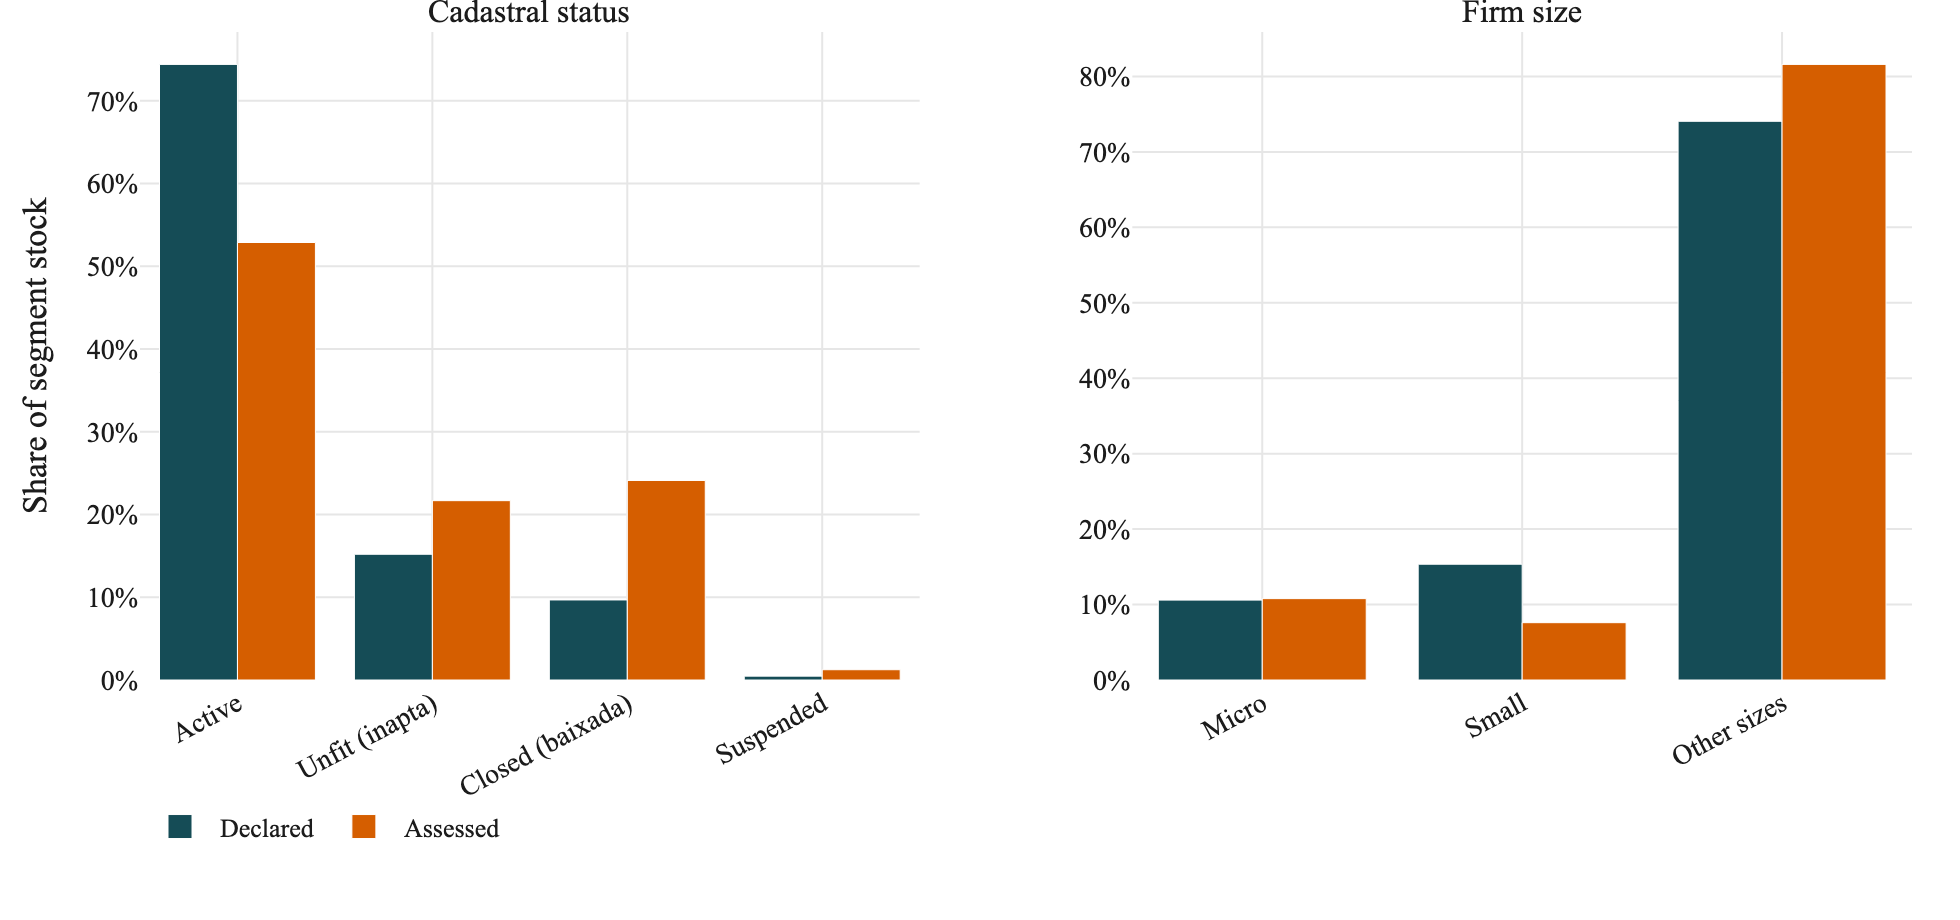
\includegraphics[width=\textwidth]{figures/fig_status_size.png}
\caption{Share of segment stock by registry status and by firm size.}\label{fig:status}
\end{figure}

\begin{figure}[t]
\centering
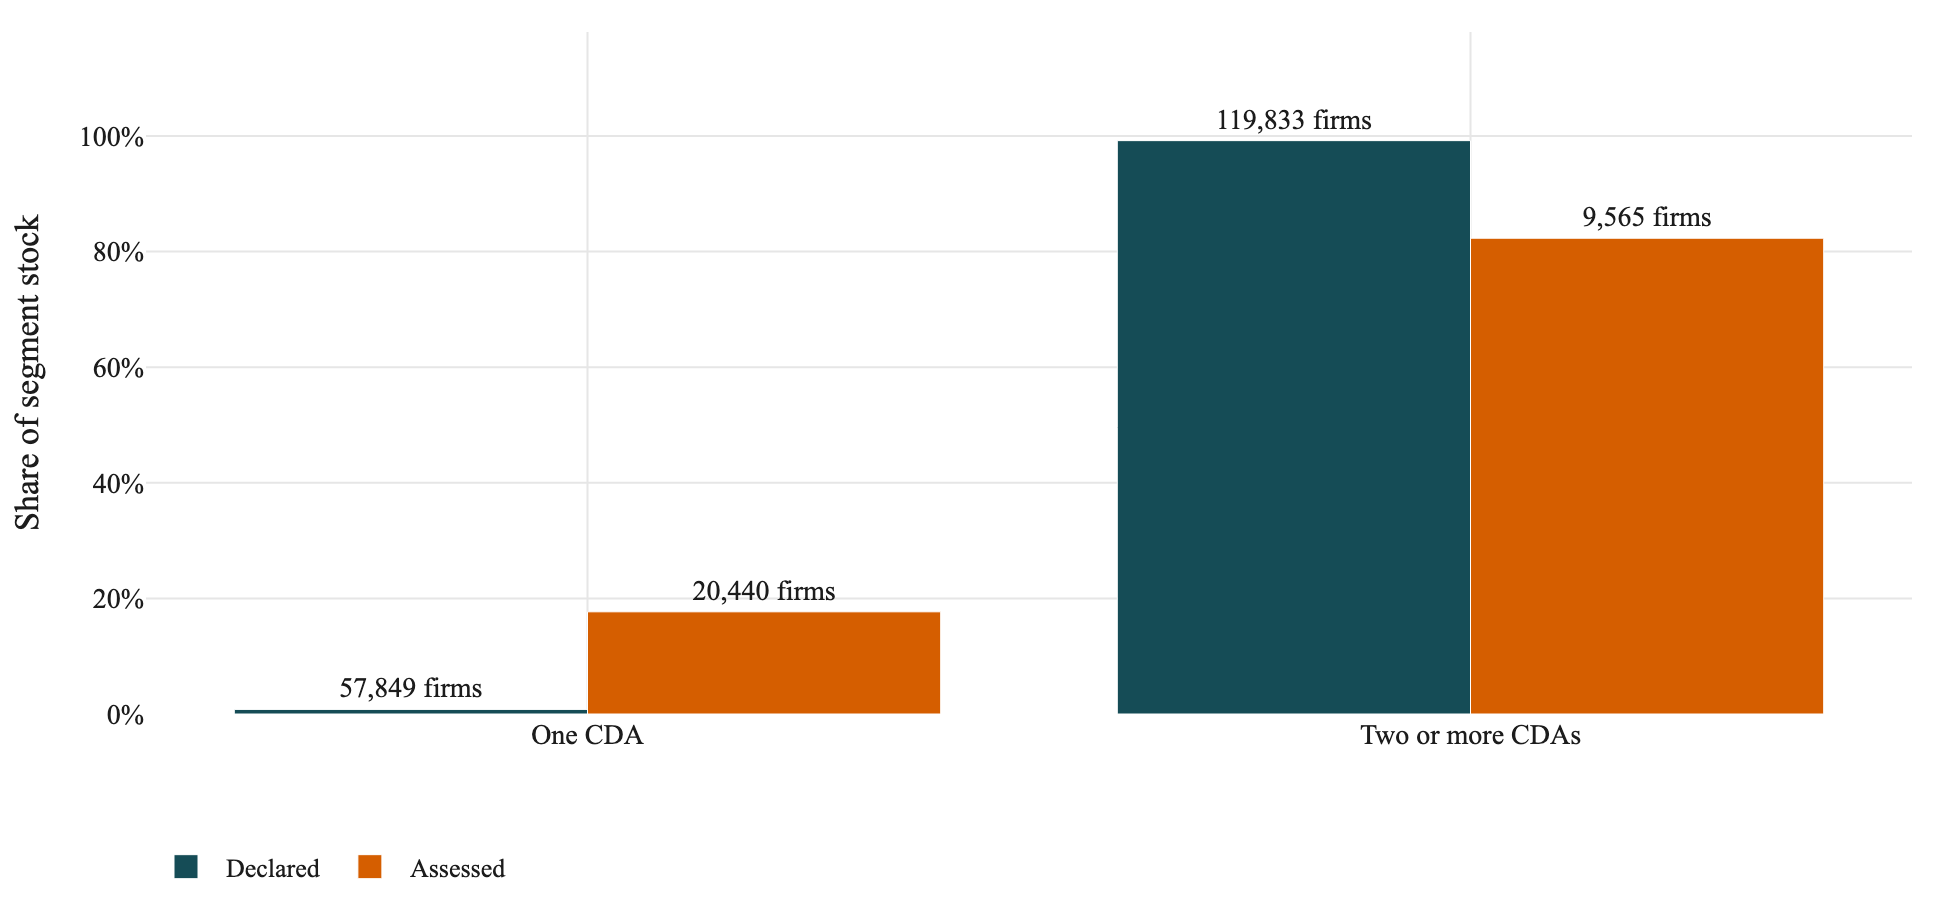
\includegraphics[width=0.92\textwidth]{figures/fig_repeated.png}
\caption{Share of segment stock held by firms with one certificate or with two or more.}\label{fig:repeated}
\end{figure}

\subsection{Selected specification and fitted associations}\label{sec:fitted}

The pre-stated cuts are applied to the estimation sample of 200,000 certificates (Section~\ref{sec:inference}).
For any payment, assessed debt keeps a linear log-stock term.
$\Delta$AIC is $-1.78$, and the spline log-odds are monotone.
Assessed debt uses a spline on debt age.
$\Delta$AIC is $25.06$, and the spline log-odds are not monotone.
Declared debt uses a spline on log stock ($\Delta$AIC $= 133.60$) and a spline on debt age ($\Delta$AIC $= 741.16$).
For the balance, the partial $R^2$ of the RESET powers is 0.016, which meets the cut of 0.01.
The rank correlation between the absolute residual and the fitted value is 0.19.
After the largest 1~percent of the estimation sample is dropped, the partial $R^2$ is 0.017.
The linear stock equation is set aside, and quantile regression is the stock equation.
For recovery, the partial $R^2$ is 0.004 and the rank correlation is 0.52, which meets the cut of 0.20.
The linear recovery equation is kept only as a comparison.
The moment intraclass correlation is 0.061 for declared municipalities and 0.014 for declared CNAE divisions.
It is 0.034 for assessed municipalities and 0.015 for assessed CNAE divisions.
A municipal random intercept therefore enters only for declared debt.
The share of groups outside the 99.8~percent funnel limits is 0.184 and 0.206.
That share does not select the mixed logit.

Those equations are fit on this cross-section.
Both payment logits converge, and both designs have full column rank.
The declared logit uses 39,972 certificates.
That count is a cap of 40,000, minus 7 certificates dropped with a small pool and 21 dropped with a separated level.
McFadden's pseudo-$R^2$ is 0.061.
The assessed logit uses 5,063 certificates, from 5,126 in the estimation sample, after 34 leave with a small pool and 29 leave with a separated level.
McFadden's pseudo-$R^2$ is 0.038.
The assessed log-stock coefficient is $-0.194$.
The HC3 interval runs from $-0.235$ to $-0.154$, so it excludes zero.
The spline basis coefficients are not slopes.
Figure~\ref{fig:partialstock} and Figure~\ref{fig:partialage} show the partial log-odds.
The vertical coordinate is the linear predictor at a grid value minus the linear predictor at the median of the fit sample.
The assessed log-stock curve is linear.
The other curves are centered splines.

\begin{figure}[H]
\centering
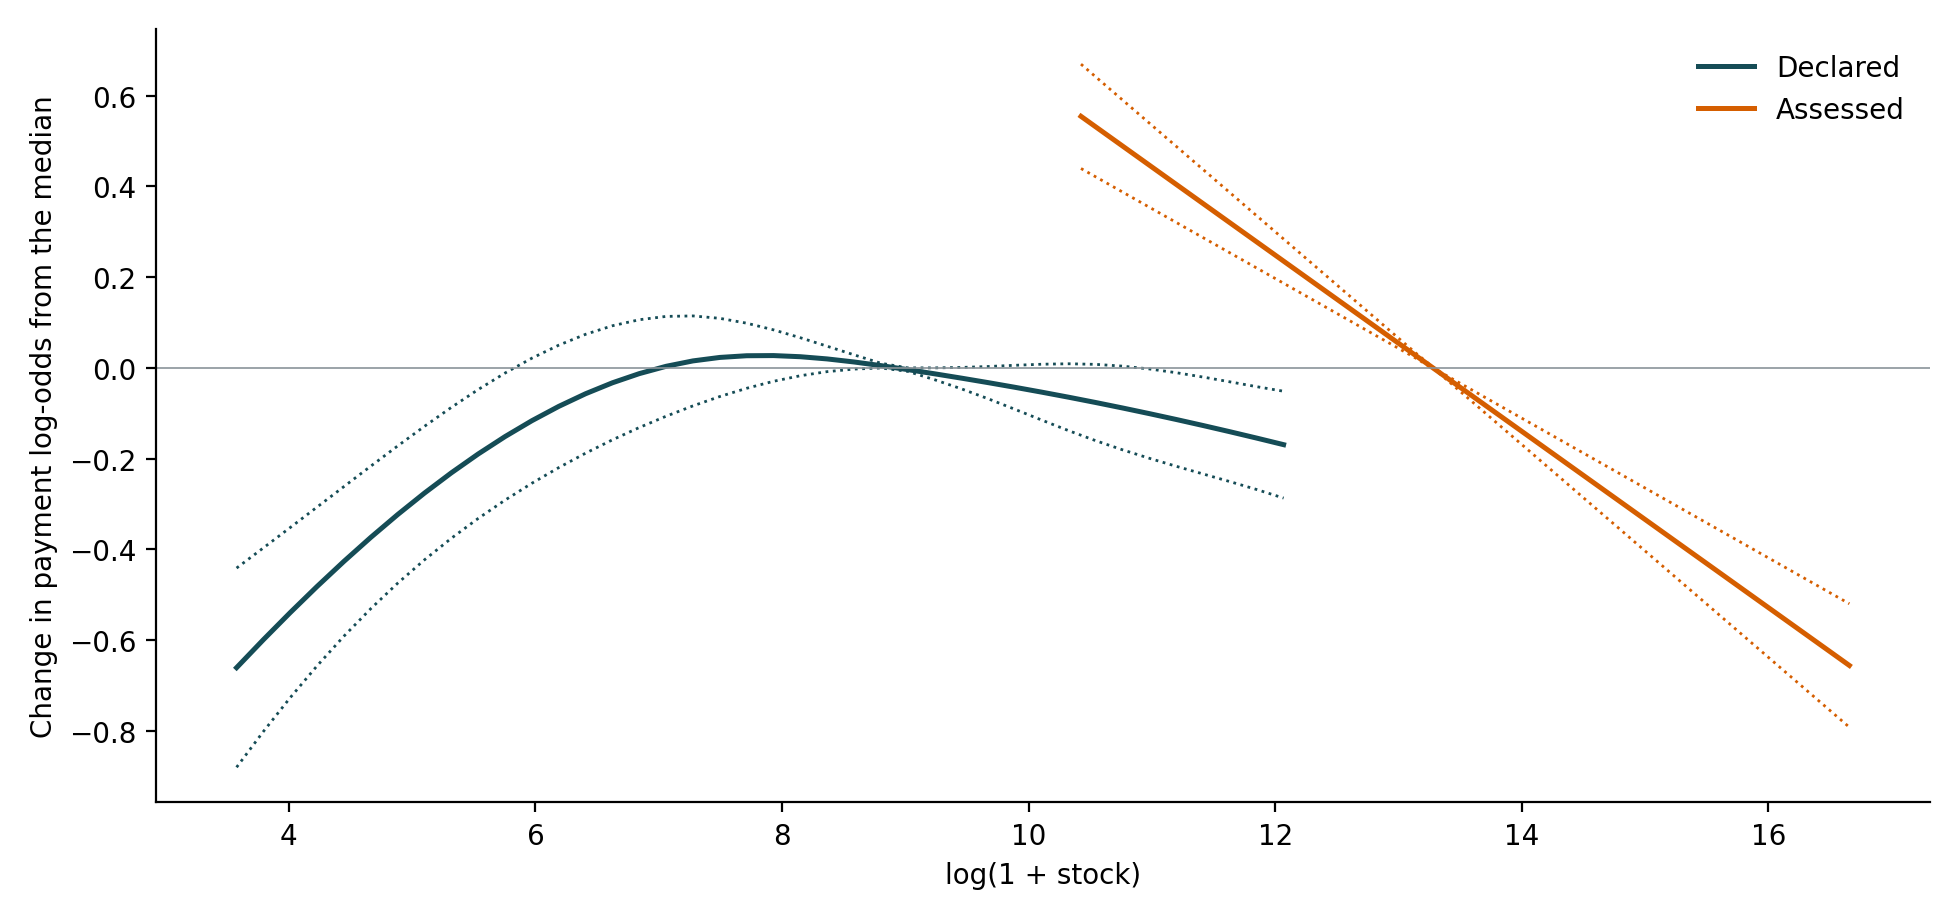
\includegraphics[width=0.88\textwidth]{figures/fig_partial_log_stock.png}
\caption{Partial payment log-odds against $\log(1+\text{stock})$. Solid lines are the point estimate. Dotted lines are the pointwise 95~percent interval. The curve is zero at the median of the fit sample.}\label{fig:partialstock}
\end{figure}

\begin{figure}[H]
\centering
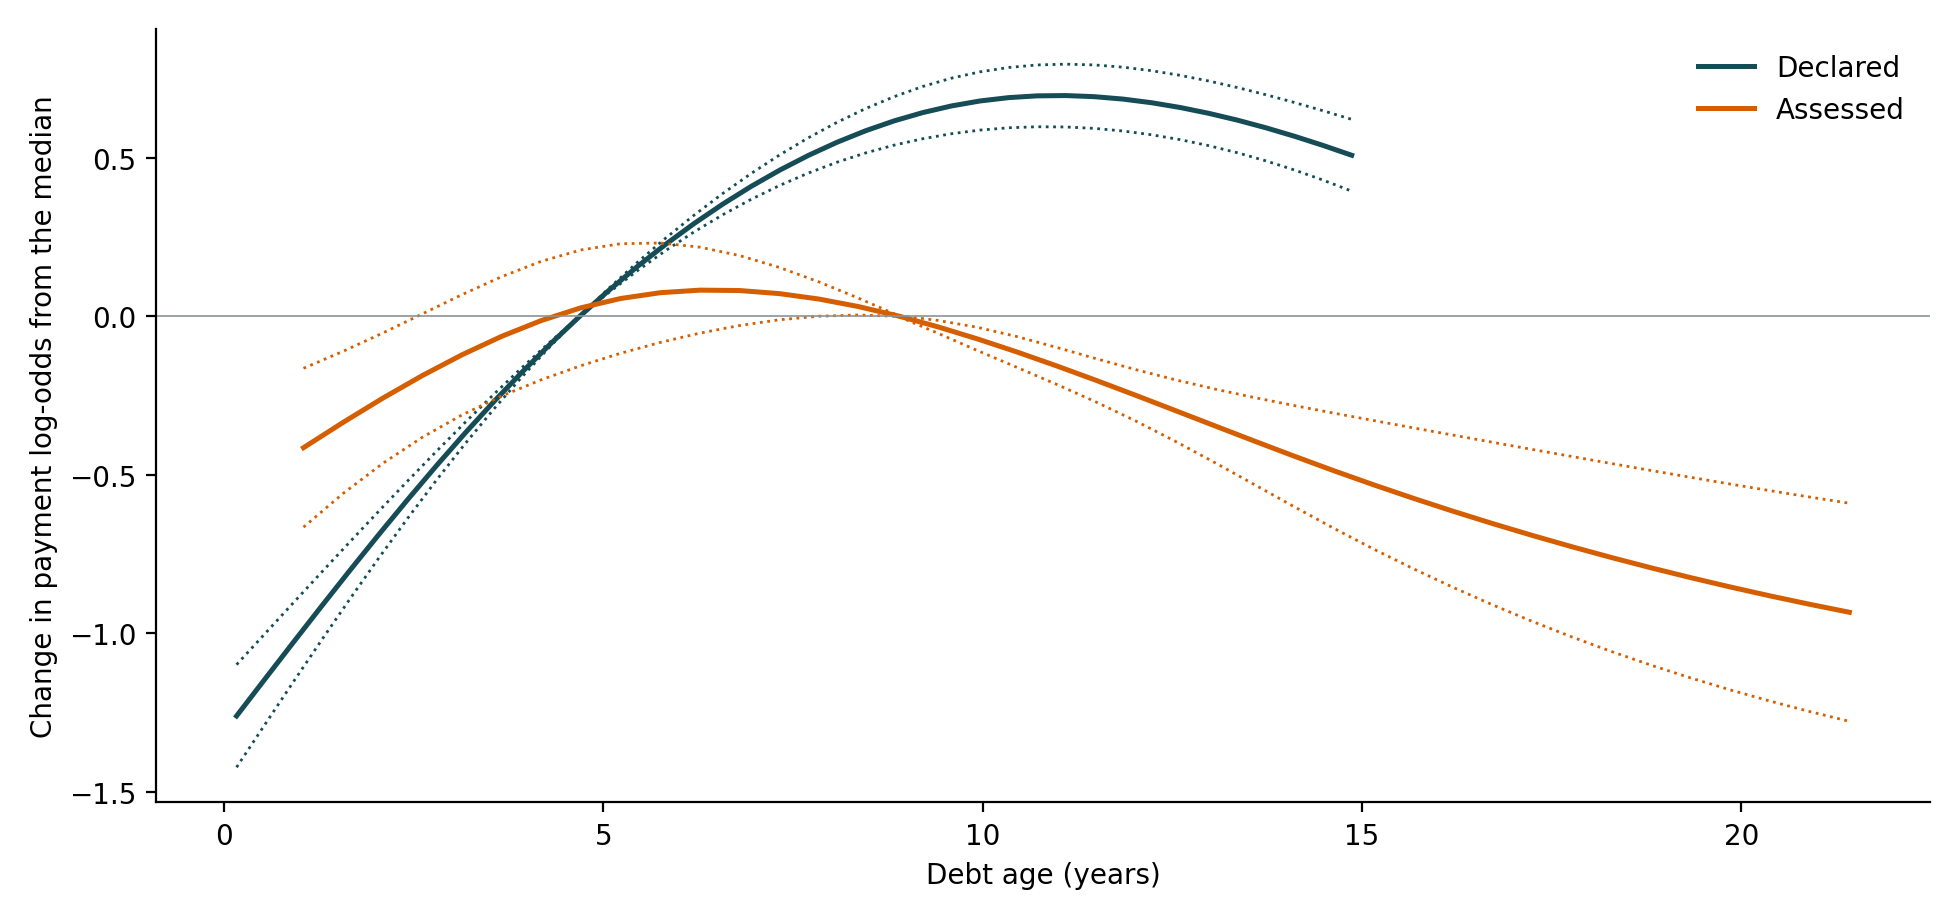
\includegraphics[width=0.88\textwidth]{figures/fig_partial_debt_age.png}
\caption{Partial payment log-odds against debt age in years. Solid lines are the point estimate. Dotted lines are the pointwise 95~percent interval. The curve is zero at the median of the fit sample.}\label{fig:partialage}
\end{figure}

The declared municipal complement uses 7,919 certificates in 670 municipalities.
The municipality standard deviation is 0.676, with an approximate posterior interval from 0.640 to 0.713.
The intraclass correlation of that fit is 0.122.
It is a property of the complement.
It is not the 0.061 screen that selected the intercept.

Table~\ref{tab:quantile} reports the debt-age coefficient in the quantile regression of log stock.
The coefficient is the change in that quantile of log stock associated with one further year of debt age, with CNAE section and firm size held fixed.
The four values of $\tau$ are four rows.
They are not a claim about the shape of the distribution.
The assessed fit uses 5,092 certificates.
The declared fit uses 19,995.

\begin{table}[t]
\centering
\caption{Debt-age coefficient in the quantile regression of $\log(1+\text{stock})$.}\label{tab:quantile}
\begin{tabular}{llrrr}
\toprule
Segment & $\tau$ & Coefficient & Interval & Certificates \\
\midrule
Assessed & 0.25 & $-0.015$ & $-0.026$ to $-0.004$ & 5,092 \\
Assessed & 0.50 & $-0.017$ & $-0.027$ to $-0.008$ & 5,092 \\
Assessed & 0.75 & $-0.022$ & $-0.032$ to $-0.011$ & 5,092 \\
Assessed & 0.90 & $-0.020$ & $-0.032$ to $-0.008$ & 5,092 \\
Declared & 0.25 & 0.213 & 0.203 to 0.223 & 19,995 \\
Declared & 0.50 & 0.140 & 0.133 to 0.147 & 19,995 \\
Declared & 0.75 & 0.091 & 0.085 to 0.098 & 19,995 \\
Declared & 0.90 & 0.069 & 0.062 to 0.076 & 19,995 \\
\bottomrule
\end{tabular}

\vspace{0.4em}
\begin{minipage}{0.95\textwidth}
\footnotesize
Notes: Rounded to the precision shown.
The interval is the default 95~percent interval of the quantile regression, not an HC3 interval.
There is no ordinary least squares column.
\end{minipage}
\end{table}

Table~\ref{tab:recoveryfit} reports the linear recovery comparison.
The outcome is the certificate ratio of payments to the December stock.
It is not the segment recovery rate in Table~\ref{tab:profile}.
On assessed debt the $R^2$ is 0.019 ($n = 5{,}092$).
On declared debt the $R^2$ is 0.0014 ($n = 194{,}709$).

\begin{table}[t]
\centering
\caption{Linear recovery comparison, HC3 intervals.}\label{tab:recoveryfit}
\begin{tabular}{llrrr}
\toprule
Segment & Term & Coefficient & HC3 interval & Certificates \\
\midrule
Assessed & Log stock & $-0.031$ & $-0.042$ to $-0.019$ & 5,092 \\
Assessed & Debt age (years) & $-0.0031$ & $-0.0047$ to $-0.0015$ & 5,092 \\
Declared & Log stock & $-0.777$ & $-1.028$ to $-0.525$ & 194,709 \\
Declared & Debt age (years) & 0.125 & 0.079 to 0.172 & 194,709 \\
\bottomrule
\end{tabular}

\vspace{0.4em}
\begin{minipage}{0.95\textwidth}
\footnotesize
Notes: Rounded to the precision shown.
Ordinary least squares of payments divided by stock, inside each segment.
This equation is a comparison with the payment logit.
It is not the stock equation.
The assessed $R^2$ is 0.019 and the declared $R^2$ is 0.0014.
\end{minipage}
\end{table}

\clearpage
Table~\ref{tab:secsize-payment}, Table~\ref{tab:secsize-mixed}, Table~\ref{tab:secsize-quantile} and Table~\ref{tab:secsize-recovery} report the section and size coefficients.

% Compact body table: key coefficients discussed in the text.
% Full list: Table~\ref{tab:app-secsize-payment} in the Online Appendix.
\begin{table}[H]
\centering
\caption{Selected section and size coefficients in the payment logit.}\label{tab:secsize-payment}
\footnotesize
\begin{tabular}{@{}llp{3.6cm}rr@{}}
\toprule
Segment & Code & Term & Coef. & HC3 95\% CI \\
\midrule
Declared & C & Manufacturing & $-0.112$ & $-0.196$ to $-0.027$ \\
Declared & H & Transportation and storage & 0.061 & $-0.055$ to 0.178 \\
Declared & J & Information and communication & 0.251 & $-0.114$ to 0.615 \\
Declared & 03 & Small & 0.033 & $-0.060$ to 0.126 \\
Declared & 05 & Other sizes & 0.154 & 0.065 to 0.244 \\
Assessed & C & Manufacturing & $-0.083$ & $-0.252$ to 0.087 \\
Assessed & H & Transportation and storage & 0.369 & 0.076 to 0.662 \\
Assessed & J & Information and communication & 0.228 & $-0.427$ to 0.883 \\
Assessed & 03 & Small & 0.267 & 0.031 to 0.503 \\
Assessed & 05 & Other sizes & 0.363 & 0.171 to 0.555 \\
\bottomrule
\end{tabular}

\vspace{0.4em}
\begin{minipage}{0.95\textwidth}
\footnotesize
Notes: Fixed-effects logit of any payment. The interval is the HC3 95~percent interval. Declared uses 39,972 certificates. Assessed uses 5,063 certificates. Trade (section G) and micro (size code 01) are the reference levels and have no coefficient. Coefficients and intervals are rounded to three decimal places. The full coefficient list is Table~\ref{tab:app-secsize-payment}.
\end{minipage}
\end{table}

% Compact body table: key coefficients discussed in the text.
% Full list: Table~\ref{tab:app-secsize-mixed} in the Online Appendix.
\begin{table}[H]
\centering
\caption{Selected section and size coefficients in the declared municipal complement.}\label{tab:secsize-mixed}
\footnotesize
\begin{tabular}{@{}lp{3.8cm}rr@{}}
\toprule
Code & Term & Coef. & Posterior 95\% CI \\
\midrule
C & Manufacturing & $-0.152$ & $-0.302$ to $-0.003$ \\
H & Transportation and storage & 0.135 & $-0.121$ to 0.392 \\
03 & Small & $-0.290$ & $-0.481$ to $-0.100$ \\
05 & Other sizes & $-0.080$ & $-0.227$ to 0.068 \\
\bottomrule
\end{tabular}

\vspace{0.4em}
\begin{minipage}{0.95\textwidth}
\footnotesize
Notes: Declared debt only, 7,919 certificates in 670 municipalities. The interval is the approximate posterior interval, not a confidence interval. Trade (section G) and micro (size code 01) are the reference levels and have no coefficient. Information and communication is not a row of this complement. Coefficients and intervals are rounded to three decimal places. The full coefficient list is Table~\ref{tab:app-secsize-mixed}.
\end{minipage}
\end{table}

% Compact body table: rows discussed in the text only.
% Full list: Table~\ref{tab:app-secsize-quantile} in the Online Appendix.
\footnotesize
\begin{longtable}{@{}lllrr@{}}
\caption{Selected section and size coefficients in the quantile regression of $\log(1+\text{stock})$.}\label{tab:secsize-quantile}\\
\toprule
Segment & $\tau$ & Term & Coef. & 95\% CI \\
\midrule
\endfirsthead
\multicolumn{5}{@{}l}{\footnotesize\textit{Continued from the previous page}}\\
\toprule
Segment & $\tau$ & Term & Coef. & 95\% CI \\
\midrule
\endhead
\midrule
\multicolumn{5}{r}{\footnotesize\textit{Continued on the next page}}\\
\endfoot
\bottomrule
\endlastfoot
Declared & 0.25 & Manufacturing & 0.966 & 0.865 to 1.067 \\
Declared & 0.50 & Manufacturing & 1.044 & 0.964 to 1.123 \\
Declared & 0.75 & Manufacturing & 0.899 & 0.824 to 0.974 \\
Declared & 0.90 & Manufacturing & 0.786 & 0.700 to 0.872 \\
Declared & 0.25 & Transportation and storage & 1.719 & 1.567 to 1.870 \\
Declared & 0.50 & Transportation and storage & 1.496 & 1.376 to 1.615 \\
Declared & 0.75 & Transportation and storage & 1.131 & 1.018 to 1.244 \\
Declared & 0.90 & Transportation and storage & 0.747 & 0.619 to 0.876 \\
Declared & 0.25 & Information and communication & 0.282 & $-0.259$ to 0.823 \\
Declared & 0.50 & Information and communication & 0.611 & 0.190 to 1.032 \\
Declared & 0.75 & Information and communication & 0.346 & $-0.049$ to 0.740 \\
Declared & 0.90 & Information and communication & 0.561 & 0.116 to 1.006 \\
Declared & 0.25 & Small & 0.561 & 0.449 to 0.672 \\
Declared & 0.50 & Small & 0.588 & 0.501 to 0.674 \\
Declared & 0.75 & Small & 0.572 & 0.491 to 0.652 \\
Declared & 0.90 & Small & 0.472 & 0.380 to 0.564 \\
Declared & 0.25 & Other sizes & 0.610 & 0.505 to 0.715 \\
Declared & 0.50 & Other sizes & 1.091 & 1.011 to 1.172 \\
Declared & 0.75 & Other sizes & 1.341 & 1.267 to 1.416 \\
Declared & 0.90 & Other sizes & 1.301 & 1.217 to 1.384 \\
Assessed & 0.25 & Manufacturing & 0.009 & $-0.143$ to 0.162 \\
Assessed & 0.50 & Manufacturing & 0.089 & $-0.057$ to 0.236 \\
Assessed & 0.75 & Manufacturing & 0.181 & 0.012 to 0.349 \\
Assessed & 0.90 & Manufacturing & 0.126 & $-0.061$ to 0.314 \\
Assessed & 0.25 & Transportation and storage & $-0.168$ & $-0.471$ to 0.135 \\
Assessed & 0.50 & Transportation and storage & $-0.328$ & $-0.619$ to $-0.036$ \\
Assessed & 0.75 & Transportation and storage & $-0.151$ & $-0.490$ to 0.187 \\
Assessed & 0.90 & Transportation and storage & $-0.222$ & $-0.605$ to 0.160 \\
Assessed & 0.25 & Information and communication & 0.910 & 0.315 to 1.506 \\
Assessed & 0.50 & Information and communication & 1.085 & 0.510 to 1.659 \\
Assessed & 0.75 & Information and communication & 0.863 & 0.205 to 1.521 \\
Assessed & 0.90 & Information and communication & 1.220 & 0.458 to 1.983 \\
Assessed & 0.25 & Small & 0.268 & 0.058 to 0.478 \\
Assessed & 0.50 & Small & 0.471 & 0.270 to 0.672 \\
Assessed & 0.75 & Small & 0.207 & $-0.026$ to 0.440 \\
Assessed & 0.90 & Small & 0.099 & $-0.165$ to 0.362 \\
Assessed & 0.25 & Other sizes & 0.846 & 0.680 to 1.012 \\
Assessed & 0.50 & Other sizes & 1.007 & 0.848 to 1.165 \\
Assessed & 0.75 & Other sizes & 0.941 & 0.758 to 1.124 \\
Assessed & 0.90 & Other sizes & 1.106 & 0.899 to 1.312 \\
\end{longtable}

\vspace{-0.6em}
\begin{minipage}{0.95\textwidth}
\footnotesize
Notes: The interval is the default 95~percent interval of the quantile regression, not an HC3 interval. Declared uses 19,995 certificates and assessed uses 5,092 certificates at each $\tau$. Trade (section G) and micro (size code 01) are the reference levels and have no coefficient. Coefficients and intervals are rounded to three decimal places. The full coefficient list is Table~\ref{tab:app-secsize-quantile}.
\end{minipage}

% Compact body table: key coefficients discussed in the text.
% Full list: Table~\ref{tab:app-secsize-recovery} in the Online Appendix.
\begin{table}[H]
\centering
\caption{Selected section and size coefficients in the linear recovery comparison.}\label{tab:secsize-recovery}
\footnotesize
\begin{tabular}{@{}llp{3.6cm}rr@{}}
\toprule
Segment & Code & Term & Coef. & HC3 95\% CI \\
\midrule
Declared & C & Manufacturing & 1.293 & 0.485 to 2.100 \\
Declared & H & Transportation and storage & 1.258 & 0.587 to 1.929 \\
Declared & J & Information and communication & 0.088 & $-0.484$ to 0.660 \\
Declared & 03 & Small & 0.187 & $-0.345$ to 0.720 \\
Declared & 05 & Other sizes & 0.627 & 0.095 to 1.159 \\
Assessed & C & Manufacturing & $-0.009$ & $-0.039$ to 0.021 \\
Assessed & H & Transportation and storage & $-0.007$ & $-0.045$ to 0.032 \\
Assessed & J & Information and communication & 0.012 & $-0.032$ to 0.056 \\
Assessed & 03 & Small & 0.036 & 0.007 to 0.066 \\
Assessed & 05 & Other sizes & 0.069 & 0.038 to 0.101 \\
\bottomrule
\end{tabular}

\vspace{0.4em}
\begin{minipage}{0.95\textwidth}
\footnotesize
Notes: Ordinary least squares of payments divided by stock, inside each segment. This equation is a comparison with the payment logit. It is not the stock equation. Declared uses 194,709 certificates. Assessed uses 5,092 certificates. Trade (section G) and micro (size code 01) are the reference levels and have no coefficient. Coefficients and intervals are rounded to three decimal places. The full coefficient list is Table~\ref{tab:app-secsize-recovery}.
\end{minipage}
\end{table}


\textbf{[DISCUTIR E ESCREVER: quais coeficientes de se\c{c}\~ao CNAE e de porte entram no texto, e a leitura dos termos de idade e de saldo.]}
